\section[Experimente]{Experimente}

\begin{frame}[<+->]
\frametitle{Rolling Stone}
\begin{minipage}[c]{0.39\textwidth}
% \vspace*{-1.5cm}
%   \includegraphics[width=\linewidth]{../dipl_tex/img/tikz/rolling-stones.pdf} \\
%   \includegraphics[width=1.05\linewidth]{../dipl_tex/img/tikz/rolling-stones-solution.pdf}
\scalebox{1.07}{\documentclass{standalone}
\IfStandalone{
	\usepackage{pgfplots,pgfplotstable}
	\usetikzlibrary{external}
	
	}{%
}
% \usepackage{pgfplots,pgfplotstable}
% \usetikzlibrary{external}
	

\begin{document}
\tikzsetnextfilename{rolling-stones}
\begin{tikzpicture}[x=3em,y=3em]
\begin{axis}[
            xmin=-2.5,xmax=2.5,
            ymin=-1.5,ymax=1.5,
            xlabel=$z$,
%             legend entries={$V(z)$,$V'(z)$},
            width=\linewidth
        ]
        \addplot[domain=-2.5:-1]{(1+x)^2/2};
        \addplot[-,domain=-1:1]{0};
        \addplot[domain=1:2.5]{(1-x)^2/2};
        \addplot[domain=-2.5:2.5,samples=100,blue]{-min(max(-1-x,0),1-x)};
\end{axis}
\end{tikzpicture}

 
\end{document}
}
\scalebox{1.2}{\documentclass{standalone}
\IfStandalone{
	\usepackage{pgfplots,pgfplotstable}
	\usetikzlibrary{external}
	
	}{%
}
\begin{document}
\tikzsetnextfilename{rolling-stones-solution}
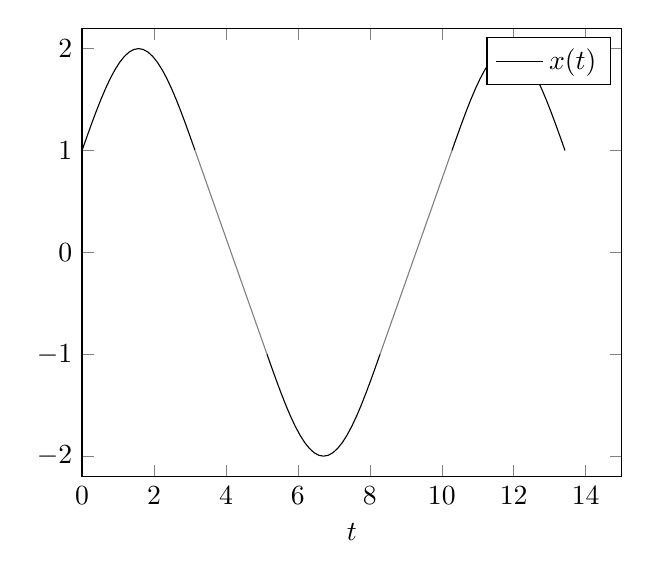
\begin{tikzpicture}[x=3em,y=3em]
\begin{axis}[
            xmin=0,xmax=15,
            ymin=-2.2,ymax=2.2,
            xlabel=$t$,
            legend entries={$x(t)$}
        ]
        \addplot[domain=0:3.14]{1+sin(deg(x))};
        \addplot[domain=pi:pi+2,gray]{1-x+pi};
        \addplot[domain=pi+2:2*pi+2]{-1-sin(deg(2-x))};
        \addplot[domain=2*pi+2:2*pi+4,gray]{x-3-2*pi};
        \addplot[domain=2*pi+4:3*pi+4]{1+sin(deg(x-2*pi-4))};
\end{axis}
\end{tikzpicture} 
\end{document}
}
\end{minipage}
\hfill
\begin{minipage}[c]{0.6\textwidth}
% \vspace*{-0.3cm}
Definiere $\ddot x = -V'(z)$ und 
\[
 V(z) = 
 \begin{cases}
 \frac{(1+z)^2}{2} & z\leq -1\\
 \frac{(1-z)^2}{2} &  z\geq 1\\
  0 & \text{sonst}
 \end{cases},
\]
$ V'(z) = \min(\max(-z-1,0),1-z)$
\pause
\begin{block}{Rolling Stone}
\centering
  $
  \begin{pmatrix}
   \dot x_1 \\
   \dot x_2 \\
  \end{pmatrix}
 = 
 \begin{pmatrix}
  x_2 \\
  -x_1 - \frac{|x_1-1|}{2} + \frac{|x_1+1|}{2}
 \end{pmatrix}
$
\end{block}
% Ist in Abs Normal Form darstellbar:
\vspace*{-0.5cm}
\pause
\[
\begin{aligned}
c = \begin{pmatrix}
     -1\\
     1
    \end{pmatrix}
& 
 Z = \begin{pmatrix}
      1 & 0 \\
      1 & 0
     \end{pmatrix} 
 \\
J = \begin{pmatrix}
      0&1\\
      -1 & 0
     \end{pmatrix}
 &
 Y = \begin{pmatrix}
      0 & 0\\
      -0.5  & 0.5
     \end{pmatrix}
\end{aligned}
\]
\end{minipage}
\end{frame}
\begin{frame}[<+->]
\frametitle{Rolling Stone Convergence}
\centering
% \includegraphics[width=0.8\linewidth]{../dipl_tex/img/tikz/convergence_rolling_plot.pdf} \\
\input{../dipl_tex/img/convergence_rolling_plot.tikz} 
\end{frame}
\begin{frame}[<+->]
\frametitle{Rolling Stone Adjungierte Gleichung}
\begin{minipage}[c]{0.45\textwidth}
\centering
% \includegraphics[width=1.02\linewidth]{../dipl_tex/img/tikz/rolling_jac_da_gradient1_imp.pdf} \\
\documentclass{standalone}
\IfStandalone{
	\usepackage{pgfplots,pgfplotstable}
	\usetikzlibrary{external}
	\newcommand{\fromRoot}[1]{../#1}
}{%
}
\begin{document}
\tikzsetnextfilename{rolling_jac_da_gradient1_imp}
\begin{tikzpicture}
    \begin{axis}[view={-20}{60}, grid=both,width=\linewidth,
%      title={$\sfrac{\partial J}{\partial x_0^{(1)}}$},
    xlabel={$x_0^{(0)}$},
    ylabel={$x_0^{(1)}$},
    zlabel={$\sfrac{\partial J}{\partial x_0^{(1)}}$}]
      \addplot3[surf] file {img/data/grad1_impl.dat};
    \end{axis}
\end{tikzpicture}
\end{document} 
(a) IMP
\end{minipage}
\begin{minipage}[c]{0.45\textwidth}
\centering
% \includegraphics[width=1.02\linewidth]{../dipl_tex/img/tikz/rolling_jac_da_gradient1.pdf} 
\input{../dipl_tex/img/rolling_jac_da_gradient1.tikz}
(b) GIMP
\end{minipage}
\hfill
\centering
\\[0.6cm]
$\xobs$ - Exakte Lösung für $x_0=(1,1)$
\end{frame}

\begin{frame}[<+->]
\frametitle{Rolling Stone Convergence}
\centering
\begin{minipage}[c]{0.49\textwidth}
\centering

% \includegraphics[width=1\linewidth]{../dipl_tex/img/tikz/rolling_convergence_adjoint_smooth.pdf} \\
\input{../dipl_tex/img/rolling_convergence_adjoint_smooth.tikz} 
(a) Glatte Observierung
\end{minipage}
\hfill
\begin{minipage}[c]{0.49\textwidth}
\centering
\documentclass{standalone}
\IfStandalone{
	\usepackage{pgfplots,pgfplotstable}
	\usetikzlibrary{external}
	\newcommand{\fromRoot}[1]{../#1}
}{%
}
\begin{document}
\tikzsetnextfilename{rolling_convergence_adjoint_discrete}
\begin{tikzpicture}
\begin{loglogaxis}[
	width=\linewidth,
	xlabel=Anzahl der Freiheitsgrade $N$,
	ylabel=Fehler in $x$,
	legend entries ={Expl. MP,
	IMP,
	GIMP, 
	}
]
  	\addplot[mark=none,red,very thin] table[x index=0,y index=3] {img/data/rolling_convergence_adjoint_discrete.dat};%expl midpoint
 	\addplot[mark=none,green,very thin] table[x index=0,y index=2] {img/data/rolling_convergence_adjoint_discrete.dat};%impl midpoint
	\addplot[mark=none,blue,very thin] table[x index=0,y index=1] {img/data/rolling_convergence_adjoint_discrete.dat};%gen midpoint

	\addplot[mark=none,very thin,gray, yshift=-20pt] 
		table[y={create col/linear regression={x=0,y=1}}] {img/data/rolling_convergence_adjoint_discrete.dat}
		  coordinate [pos=0.2] (A)
		  coordinate [pos=0.3] (B)
		;
	% save the slope parameter:
	\pgfmathparse{-\pgfplotstableregressiona}	
	\pgfmathsetmacro{\slope}{\pgfmathresult}
	
	% draw the opposite and adjacent sides
	% of the triangle
	\draw[very thin,gray] (B) -| (A)
	node [pos=0.2,anchor=north]
	{\pgfmathprintnumber{\slope}};
\end{loglogaxis}
\end{tikzpicture}
\end{document} 
% \includegraphics[width=1\linewidth]{../dipl_tex/img/tikz/rolling_convergence_adjoint_discrete.pdf} \\
(b) Diskrete Observierung
\end{minipage}

\end{frame}

\begin{frame}[<+->]
\frametitle{Rolling Stone Optimierung}
\begin{minipage}[c]{0.49\textwidth}
\centering
% \includegraphics[width=1.02\linewidth]{../dipl_tex/img/tikz/rolling_opt2_cost.pdf} \\
\documentclass{standalone}
\usepackage{pgfplots,pgfplotstable}
\IfStandalone{
	\usepackage{pgfplots,pgfplotstable}
	\usetikzlibrary{external}
	\newcommand{\fromRoot}[1]{../#1}
}{%
}
\begin{document}
\tikzsetnextfilename{rolling_opt2_cost}
\begin{tikzpicture}
    \begin{axis}[view={0}{90},
    width=\linewidth,
    legend entries ={Kostenfunktional,IMP, GIMP},
    legend style={at={(0.97,1.40)}},
%     legend style={at={(1.00,0.15)},anchor=east}
    xlabel={$x_0^{(0)}$},
    ylabel={$x_0^{(1)}$},
    zlabel={$\sfrac{\partial J}{\partial x_0^{(1)}}$}]
%     \addplot3[surf] file {img/data/rolling_costfunctional.dat};
     \addplot3[contour gnuplot={number=5}] file {img/data/rolling_costfunctional.dat};
    \addplot3[mark=o, green] table {img/data/rolling_opt2_iterationSteps_impl.dat};
    \addplot3[mark=o, blue] table {img/data/rolling_opt2_iterationSteps.dat};
    \end{axis}
\end{tikzpicture}
\end{document} 
\end{minipage}
\hfill
\begin{minipage}[c]{0.49\textwidth}
\centering
% \includegraphics[width=1.02\linewidth]{../dipl_tex/img/tikz/rolling_opt2_convergence.pdf} 
\documentclass{standalone}
\usepackage{pgfplots,pgfplotstable}
\IfStandalone{
	\usepackage{pgfplots,pgfplotstable}
	\usetikzlibrary{external}
	\newcommand{\fromRoot}[1]{../#1}
}{%
}
\begin{document}
\tikzsetnextfilename{rolling_opt2_convergence}
\begin{tikzpicture}
\begin{loglogaxis}[
	width=\linewidth,
	xlabel=Optimierungsschritte,
	ylabel=Fehler,
% 	title=Convergence of Optimization for Rolling Stones,
	legend entries ={GIMP,IMP},
	legend style={at={(0.87,1.28)}}
]
  	\addplot[mark=none,red,very thin] table[x index=0,y index=1] {img/data/rolling_opt2_convergence.dat};%gen midpoint
 	\addplot[mark=none,yellow,very thin] table[x index=0,y index=2] {img/data/rolling_opt2_convergence.dat};%impl midpoint
\end{loglogaxis}
\end{tikzpicture}

\end{document}  
\end{minipage}
\centering
$
x_0^{(\text{Start})}=(0,-1.45) 
$

\end{frame}


\begin{frame}[<+->]
\frametitle{LC Diode}
    
    Experimente

\end{frame}

\begin{frame}[<+->]
\frametitle{Shallow Water Equation}
    
    Experimente

\end{frame}